% lint-skip: 未完成ステータス（figure/table caption 未対応，人手チェック時に解消予定）
\documentclass[../../main.tex]{subfiles}
\begin{document}

\begin{flushright}
  \footnotesize\textit{【自動文字起こし・要確認】}
\end{flushright}

\noindent
[\textbf{解1}] $O$ を原点とし，$B$ が $x$ 軸上，$A$ が第一象限になるよう $xy$ 平面をおく．
この時 $|\vec{a}| = a$, $|\vec{b}| = b$ とすると，$\angle AOB = \dfrac{\pi}{3}$ より，
\[
  \vec{b} = b
  \begin{pmatrix} 1 \\ 0
  \end{pmatrix}, \quad \vec{a} = \dfrac{a}{2}
  \begin{pmatrix} 1 \\ \sqrt{3}
  \end{pmatrix}
\]
とおける．$AB$ の中点を $M$ とする．
\[
  \vec{AB} =
  \begin{pmatrix} b - \dfrac{1}{2}a \\ -\dfrac{\sqrt{3}}{2}a
  \end{pmatrix}
\]
だから，$|MC| = \dfrac{\sqrt{3}}{2}|AB|$, $MC \perp AB$, $C$ が $O$ と反対側であることをあわせて，
\[
  \vec{MC} = \dfrac{\sqrt{3}}{2}
  \begin{pmatrix} \dfrac{\sqrt{3}}{2}a \\ b - \dfrac{1}{2}a
  \end{pmatrix}
\]
となり，
\begin{align}
  \vec{c} &= \vec{OM} + \vec{MC} \\
  &= a
  \begin{pmatrix} 1 \\ 0
  \end{pmatrix} + \dfrac{1}{2}b
  \begin{pmatrix} 1 \\ \sqrt{3}
  \end{pmatrix} \quad \dots \text{①}
\end{align}
一方，
\[
  \dfrac{b}{a}\vec{a} + \dfrac{a}{b}\vec{b} = b \cdot \dfrac{1}{2}
  \begin{pmatrix} 1 \\ \sqrt{3}
  \end{pmatrix} + a
  \begin{pmatrix} 1 \\ 0
  \end{pmatrix} \quad \dots \text{②}
\]
①, ②から
\[
  \vec{c} = \dfrac{b}{a}\vec{a} + \dfrac{a}{b}\vec{b}
\]
となる．

\begin{figure}[htb]
  \centering
  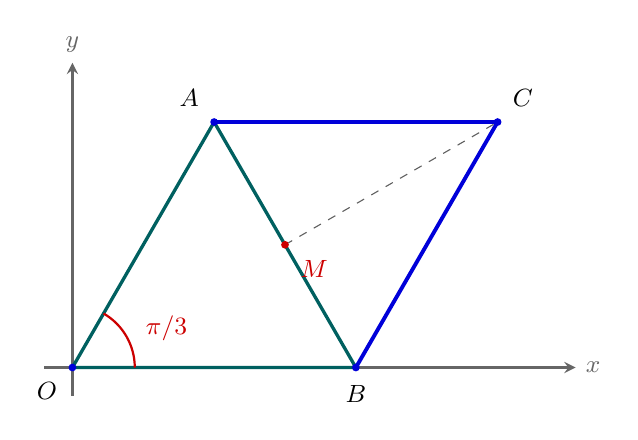
\begin{tikzpicture}[x=1.8cm, y=1.8cm, >=stealth,
    every node/.style={font=\small}]
    % OA = OB = 2, so C = (3, sqrt(3)) makes ABC equilateral.
    \coordinate (O) at (0,0);
    \coordinate (A) at (1,{sqrt(3)});
    \coordinate (B) at (2,0);
    \coordinate (M) at (1.5,{sqrt(3)/2});
    \coordinate (C) at (3,{sqrt(3)});

    \draw[->, thick, gray!80!black] (-0.2,0) -- (3.55,0) node[right] {$x$};
    \draw[->, thick, gray!80!black] (0,-0.2) -- (0,2.15) node[above] {$y$};
    \draw[line width=1.2pt, teal!75!black] (O) -- (A) -- (B) -- cycle;
    \draw[line width=1.4pt, blue!85!black] (A) -- (C) -- (B);
    \draw[dashed, gray!75!black] (M) -- (C);
    \draw[red!80!black, thick] (0.44,0) arc[start angle=0,end angle=60,radius=0.44];
    \node[red!80!black, right] at (0.45,0.28) {$\pi/3$};

    \foreach \P in {O,A,B,C} {\fill[blue!85!black] (\P) circle (1.4pt);}
    \fill[red!80!black] (M) circle (1.4pt);
    \node[below left=2pt] at (O) {$O$};
    \node[above left=2pt] at (A) {$A$};
    \node[below=3pt] at (B) {$B$};
    \node[above right=2pt] at (C) {$C$};
    \node[below right=2pt, red!80!black] at (M) {$M$};
  \end{tikzpicture}
  \caption{$AB$ の中点 $M$ と，$O$ と反対側にある正三角形 $ABC$ の頂点 $C$}
\end{figure}

\noindent
[\textbf{解2}] $\vec{a}, \vec{b}$ に平行な単位ベクトルを $\vec{x}, \vec{y}$ とすると，これらは1次独立で，又 $\vec{x} \cdot \vec{y} = \dfrac{1}{2}$ となる．さらに
\[
  \vec{c} = \alpha \vec{x} + \beta \vec{y}
\]
とおける．
\begin{align}
  \vec{AB} &= |\vec{b}|\vec{y} - |\vec{a}|\vec{x} \\
  \vec{AC} &= (\alpha - |\vec{a}|)\vec{x} + \beta \vec{y} \\
  \vec{BC} &= \alpha \vec{x} + (\beta - |\vec{b}|)\vec{y}
\end{align}
これらの大きさ2乗が全て等しいので，$k \ge 0$ として
\[
  \begin{cases}
    |\vec{b}|^2 + |\vec{a}|^2 - |\vec{a}||\vec{b}| = k \\
    (\alpha - |\vec{a}|)^2 + \beta^2 + \beta(\alpha - |\vec{a}|) = k \\
    \alpha^2 + (\beta - |\vec{b}|)^2 + \alpha(\beta - |\vec{b}|) = k
  \end{cases}
  \quad \dots (*)
\]
$(\alpha, \beta) = (|\vec{b}|, |\vec{a}|)$ とすると，(*)は成立する．又，$\vec{x}, \vec{y}$ は1次独立であることから，コレ以外の解には他ならず，
\begin{align}
  \vec{c} &= |\vec{b}|\vec{x} + |\vec{a}|\vec{y} \\
  &= |\vec{b}|\dfrac{\vec{a}}{|\vec{a}|} + |\vec{a}|\dfrac{\vec{b}}{|\vec{b}|}
\end{align}
である．

\newpage

\end{document}
